\chapter{CSS and JavaScript}\index{CSS}\index{JavaScript}

At the end of the HTML chapter, you had a complete recipe page for chocolate chip cookies. It works,
but it looks like a web page from 1995: black Times New Roman on white, blue underlined links, and a
table with clunky double borders. Nobody would send that to a friend.

In this chapter, you will turn that page into something you would be proud to show off. You will use
\newterm{CSS} to give it colors, fonts, rounded buttons, and a layout that works on both a laptop and a
phone. Then you will use \newterm{JavaScript} to make it respond to clicks: a dark mode button, steps
you can cross off as you bake, and a box that doubles or triples the recipe. Finally, you will serve the
page from your own Express server, like the one you built in the Building a Web API chapter, and add a like
button that counts likes from everyone who visits.

\begin{figure}[htbp]
\centering
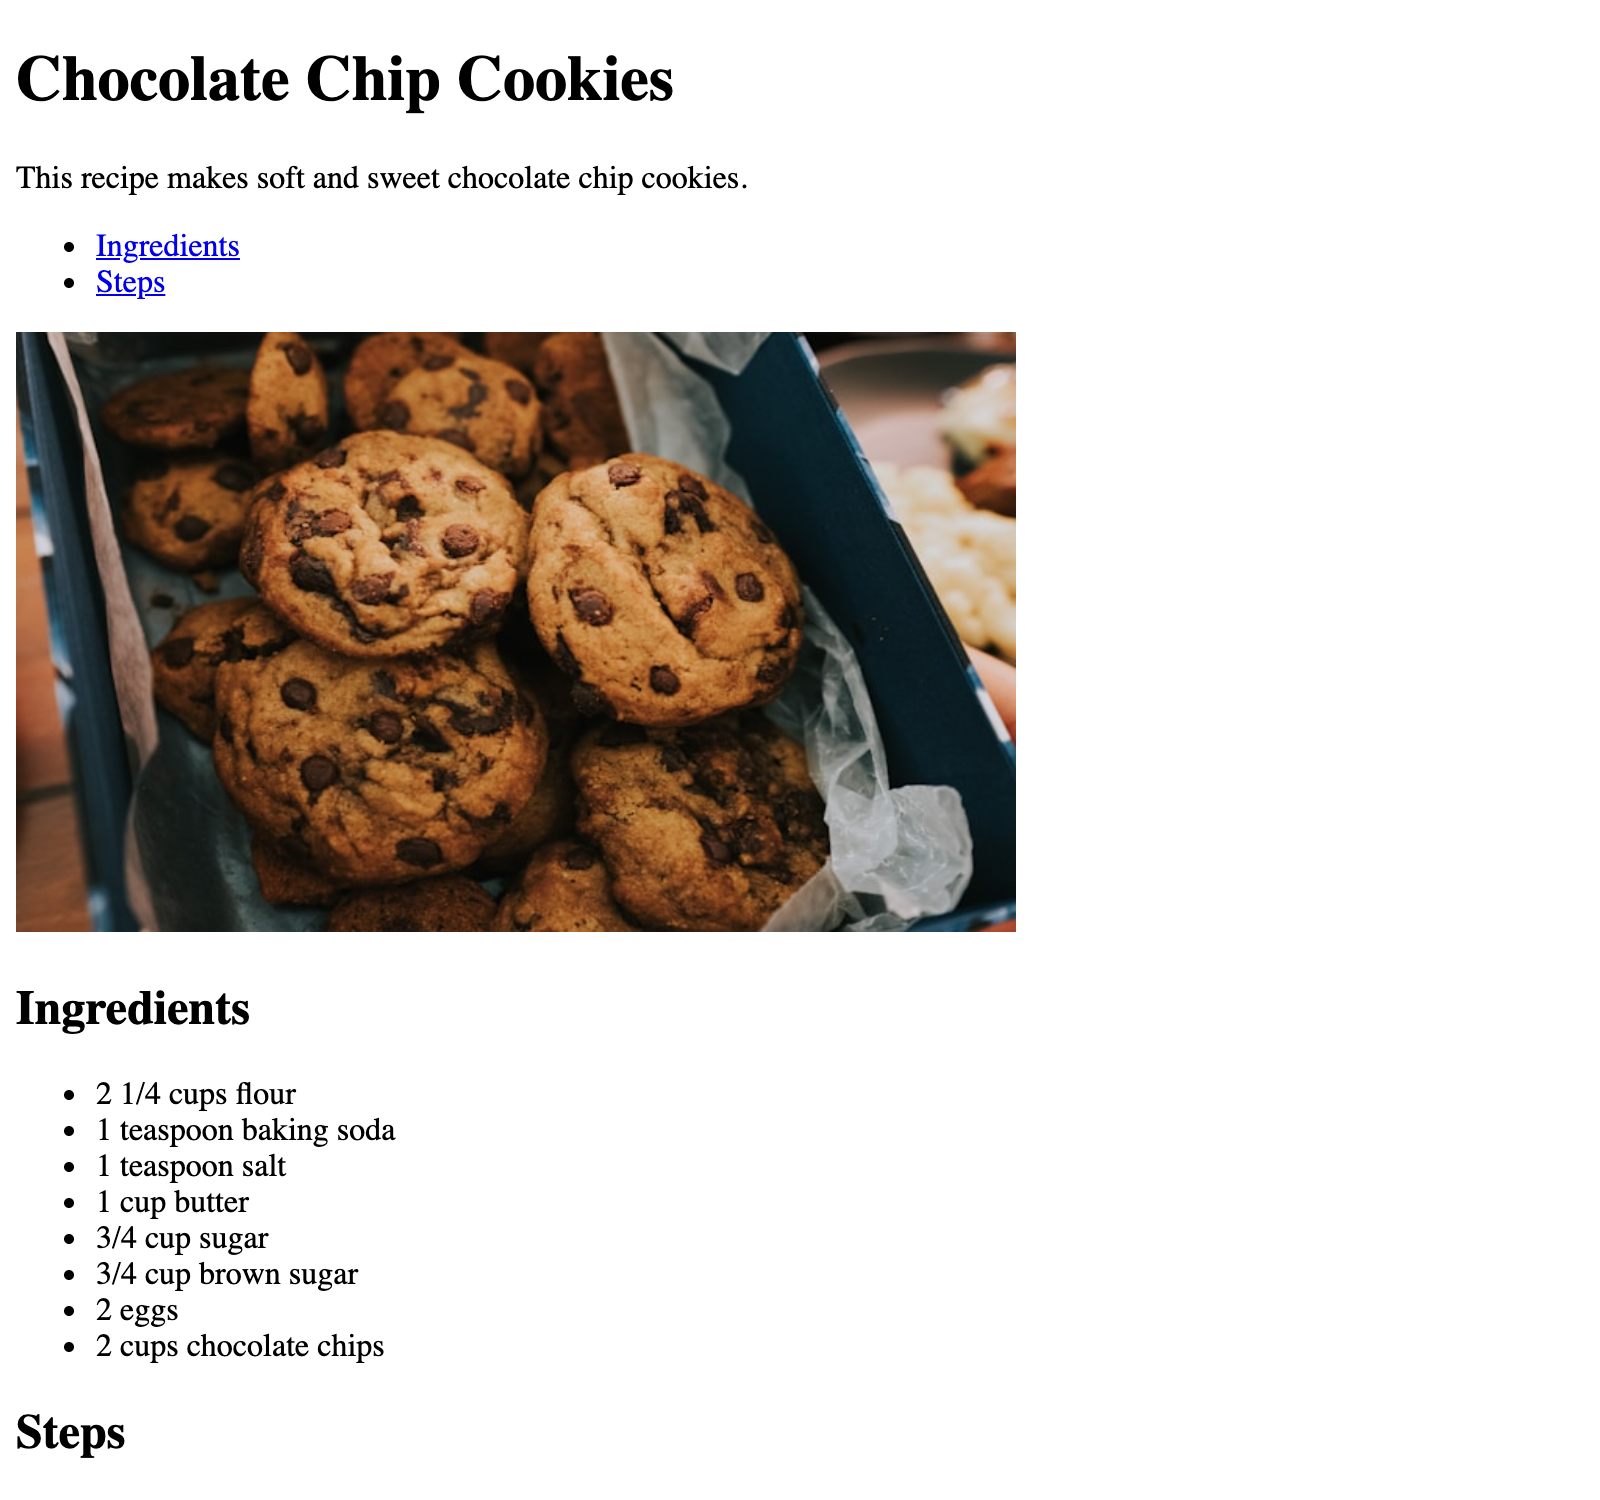
\includegraphics[width=0.48\textwidth]{recipe_before.png}\hfill
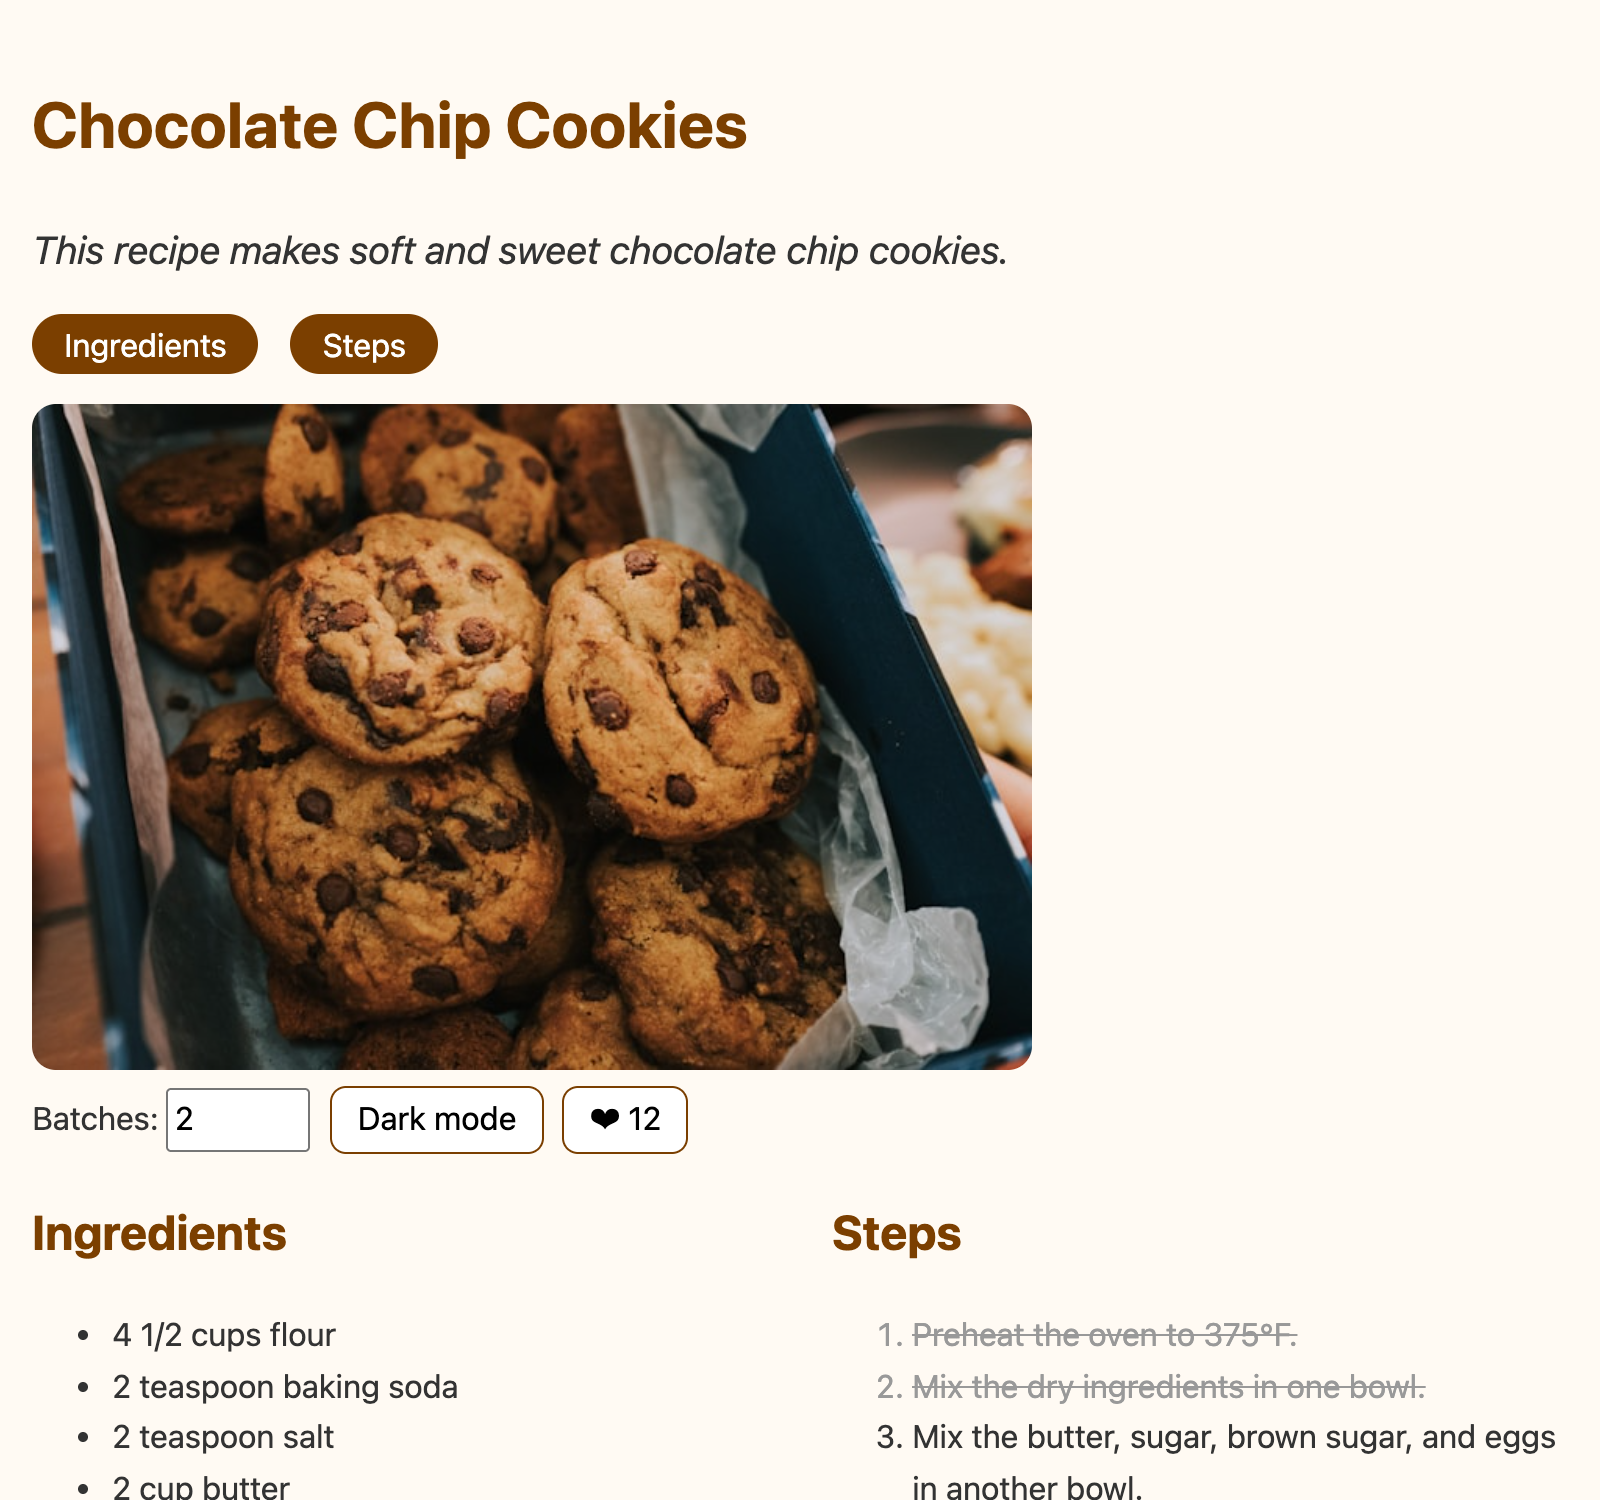
\includegraphics[width=0.48\textwidth]{recipe_after.png}
\caption{The recipe page at the end of the HTML chapter (left) and at the end of this chapter (right),
with the recipe doubled and the first two steps crossed off.}
\label{fig:recipe-before-after}
\end{figure}

\section{Setting Up}
Make a folder called \filename{recipe}, and inside it, a folder called \filename{public}. Into
\filename{public}, put the finished page from the end of the HTML chapter, saved as
\filename{index.html}, along with \filename{cookies.jpg}. By the end of the chapter, the project will
look like this:

\begin{verbatim}
recipe/
    server.js          the Express server
    public/
        index.html     the structure (HTML)
        style.css      the looks (CSS)
        script.js      the behavior (JavaScript)
        cookies.jpg
\end{verbatim}

Keeping the three languages in three files is a good habit. When something looks wrong, you know to
look in \filename{style.css}; when a button does nothing, you know to look in \filename{script.js}.

Until the last section, you do not need a server. Just double-click \filename{index.html} to open it in
your browser, and press reload each time you save a change.

\section{Your First Stylesheet}
A CSS file is a list of \newterm{rules}. Each rule picks some elements with a \newterm{selector}, then
sets \newterm{properties} on them:\index{CSS!rule}\index{CSS!selector}

\begin{minted}{css}
selector {
  property: value;
  another-property: value;
}
\end{minted}

Create \filename{style.css} in the \filename{public} folder, and start with these rules:

\begin{minted}{css}
body {
  font-family: system-ui, sans-serif;
  line-height: 1.6;
  color: #333333;
  background-color: #fffaf3;
  max-width: 800px;
  margin: 0 auto;
  padding: 1rem;
}

h1, h2 {
  color: #7b3f00;
}

.intro {
  font-size: 1.2rem;
  font-style: italic;
}
\end{minted}

To connect the stylesheet to the page, add a \verb|<link>| element to the \verb|<head>| of
\filename{index.html}:

\begin{minted}{html}
<link rel="stylesheet" href="style.css">
\end{minted}

Reload the page. The text switches to your computer's own interface font (\verb|system-ui|), the
background turns a warm cream, the headings turn chocolate brown, and the whole page sits in a centered
column instead of stretching across a wide screen.

A few things to notice:
\begin{itemize}
\item \textbf{Colors} are hex codes, just like the ones in the Data Representation chapter: \verb|#7b3f00|
means red \verb|7b|, green \verb|3f|, blue \verb|00|. CSS also understands about 140 color names, such as
\verb|white| and \verb|tomato|.
\item \textbf{Sizes} come in units. \verb|px| is a pixel. \verb|rem| is the height of the page's normal
text, so \verb|1.2rem| is 20\% bigger than normal. \verb|line-height: 1.6| (no unit) means each line takes
1.6 times the height of the text, which makes paragraphs easier to read.
\item \verb|margin: 0 auto| sets the top and bottom margins to 0 and lets the browser split the leftover
space equally on the left and right. That is the classic trick for centering a column.
\end{itemize}

You may remember the \verb|style| attribute from the HTML chapter, which puts CSS directly on one element.
It works, but a separate stylesheet lets one rule restyle every page on your site at once.

\section{Selectors and the Cascade}\index{CSS!cascade}
Selectors are how CSS finds elements. These are the ones you will use most:

\begin{center}
\begin{tabular}{l l}
Selector & Picks \\
\hline
\verb|h2| & every \verb|<h2>| element \\
\verb|.intro| & every element with \verb|class="intro"| \\
\verb|#batches| & the one element with \verb|id="batches"| \\
\verb|h1, h2| & every \verb|<h1>| and every \verb|<h2>| \\
\verb|nav a| & every \verb|<a>| inside a \verb|<nav>| \\
\verb|a:hover| & a link while the mouse is over it \\
\end{tabular}
\end{center}

Now you can see why the HTML chapter had you give elements \verb|class| and \verb|id| attributes: they
are handles for CSS and JavaScript to grab.

What if two rules disagree? The name ``Cascading Style Sheets'' refers to the answer. The more
\emph{specific} selector wins: an id beats a class, and a class beats a plain element name. If two
selectors are equally specific, the one that comes later in the file wins.

\section{The Box Model}\index{CSS!box model}
To CSS, every element is a rectangle. Around its content are three layers: \newterm{padding} (space
inside the border), the \newterm{border} itself, and \newterm{margin} (space outside the border, pushing
other elements away).

\begin{figure}[htbp]
\centering
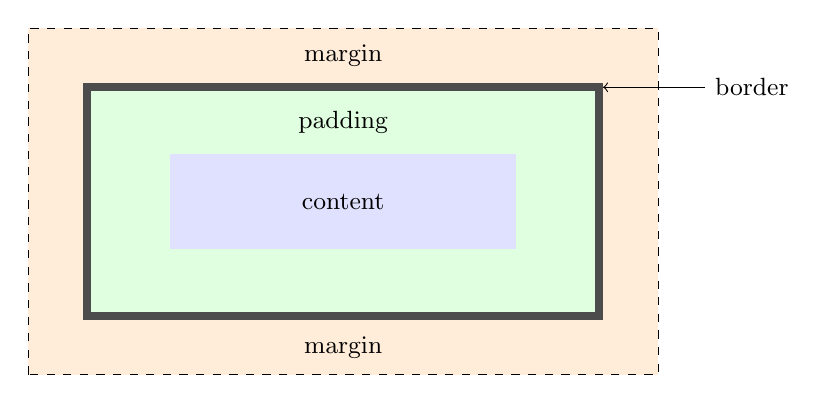
\begin{tikzpicture}[font=\small]
  \fill[orange!15] (0,0) rectangle (8,4.4);
  \fill[black!70] (0.7,0.7) rectangle (7.3,3.7);
  \fill[green!12] (0.8,0.8) rectangle (7.2,3.6);
  \fill[blue!12] (1.8,1.6) rectangle (6.2,2.8);
  \draw[dashed] (0,0) rectangle (8,4.4);
  \node at (4,2.2) {content};
  \node at (4,3.2) {padding};
  \node at (4,4.05) {margin};
  \node at (4,0.35) {margin};
  \draw[->] (8.6,3.65) node[right]{border} -- (7.3,3.65);
\end{tikzpicture}
\caption{The box model. A background color fills the content and padding; the margin is always
transparent.}
\label{fig:box-model}
\end{figure}

Two rules from our stylesheet use the box model to fix the clunky table and the photo:

\begin{minted}{css}
img {
  max-width: 100%;
  height: auto;
  border-radius: 12px;
}

table {
  border-collapse: collapse;
}

td {
  border: 1px solid #d2b48c;
  padding: 0.4rem 0.8rem;
}
\end{minted}

\verb|border: 1px solid #d2b48c| gives each cell a thin tan line, and \verb|border-collapse| merges
neighboring cells' borders into one. Now you can delete the old-fashioned \verb|border="1"| attribute from
the \verb|<table>| tag. The padding gives the words in each cell room to breathe.

The image rule matters on phones. The \verb|<img>| tag asks for a width of 500 pixels, which is wider than
many phone screens. \verb|max-width: 100%| says ``never wider than the space you are in,'' and
\verb|height: auto| keeps the photo's proportions. \verb|border-radius| rounds the corners.

\section{Layout with Flexbox}\index{CSS!flexbox}
By default, elements stack from top to bottom. To line things up side by side, use
\newterm{flexbox}. Setting \verb|display: flex| on a container lays its children out in a row.

Start with the navigation links, which are currently a bulleted list. These rules turn them into a row of
rounded buttons:

\begin{minted}{css}
nav ul {
  display: flex;
  gap: 1rem;
  list-style: none;
  padding: 0;
}

nav a {
  background-color: #7b3f00;
  color: white;
  text-decoration: none;
  padding: 0.4rem 1rem;
  border-radius: 999px;
}

nav a:hover {
  background-color: #a0522d;
}
\end{minted}

\verb|list-style: none| removes the bullets, \verb|text-decoration: none| removes the underlines, and a
huge \verb|border-radius| turns each rectangle into a pill. The \verb|:hover| rule makes a button lighten
when the mouse is over it, which tells the user it is clickable.

Next, put the ingredients and steps side by side, but only when there is room:

\begin{minted}{css}
main {
  display: flex;
  flex-wrap: wrap;
  gap: 2rem;
}

main section {
  flex: 1 1 250px;
}
\end{minted}

\verb|flex: 1 1 250px| says each section would like to be 250 pixels wide, may grow to share extra space,
and may shrink. \verb|flex-wrap: wrap| lets sections that do not fit move to the next row. On a laptop,
ingredients and steps sit next to each other; on a phone, they stack. A page that rearranges itself for
the screen it is on is called \newterm{responsive}.\index{responsive design} (It also needs the
\verb|viewport| meta tag from the HTML chapter, which tells phones not to pretend to be a wide screen.)

\begin{figure}[htbp]
\centering
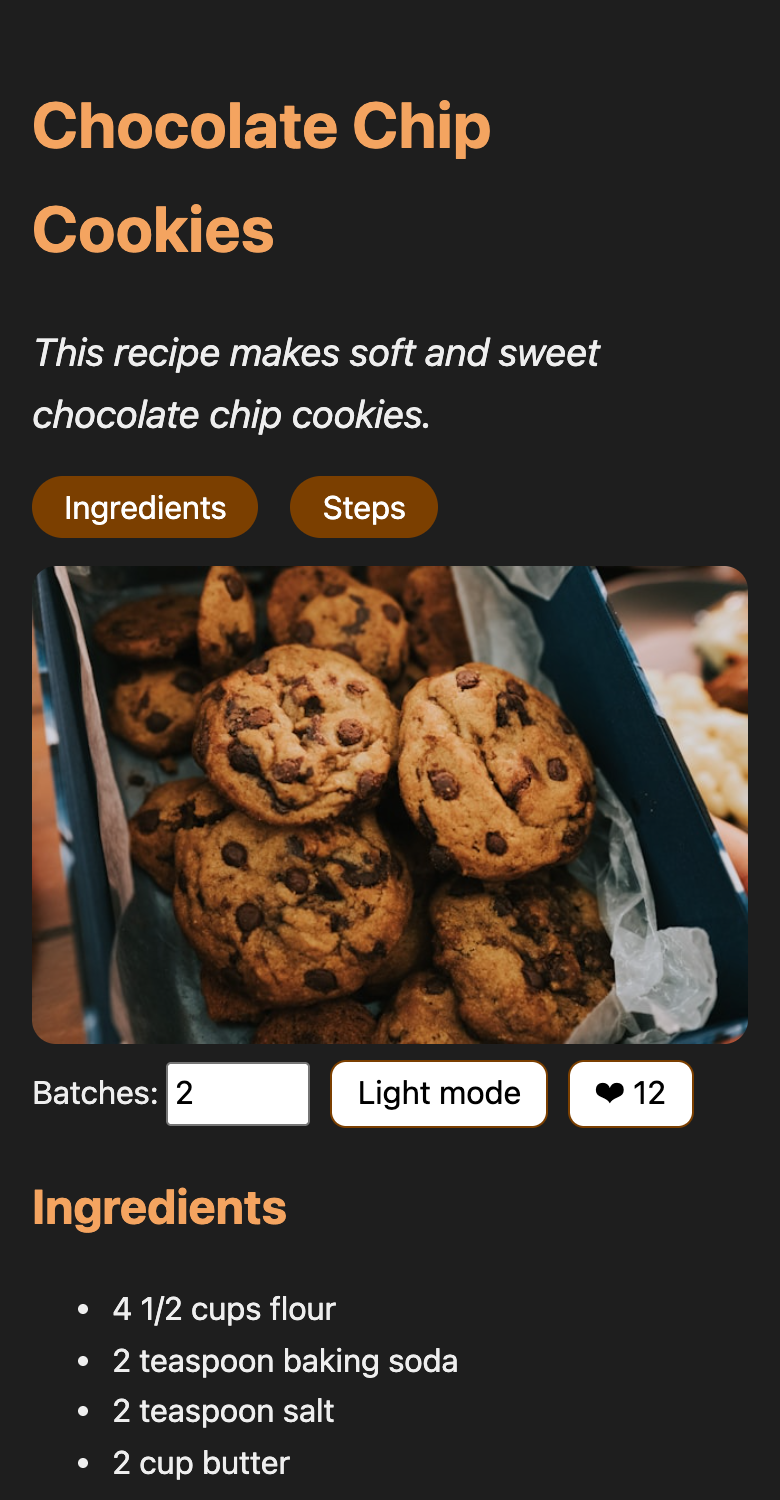
\includegraphics[width=0.4\textwidth]{recipe_phone_dark.png}
\caption{The same page on a phone, in dark mode. The ingredients and steps now stack.}
\label{fig:recipe-phone}
\end{figure}

\section{JavaScript for Python Programmers}
CSS controls how the page looks. To make it \emph{do} things, you need a programming language that runs
inside the browser, and there is only one: JavaScript. You have already seen some in the Building a Web API
chapter, where your Express server was written in it. Since you know Python (and some C), most of
JavaScript will look familiar:

\begin{center}
\begin{tabular}{l l}
Python & JavaScript \\
\hline
\verb|x = 5| & \verb|let x = 5;| \\
 & \verb|const y = 10;| (cannot be reassigned) \\
\verb|print("hi", x)| & \verb|console.log("hi", x);| \\
\verb|if x > 3:| & \verb|if (x > 3) { ... }| \\
\verb|elif|, \verb|else| & \verb|else if|, \verb|else| \\
\verb|for item in items:| & \verb|for (const item of items) { ... }| \\
\verb|def area(r):| & \verb|function area(r) { ... }| \\
\verb|[1, 2, 3]| (list) & \verb|[1, 2, 3]| (array) \\
\verb|{"likes": 3}| (dict) & \verb|{ likes: 3 }| (object) \\
\verb|and|, \verb|or|, \verb|not| & \verb|&&|, \verb+||+, \verb|!| \\
\verb|==| & \verb|===| \\
\verb|True|, \verb|False|, \verb|None| & \verb|true|, \verb|false|, \verb|null| \\
\end{tabular}
\end{center}

The biggest differences: blocks are marked with curly braces instead of indentation (as in C),
statements end with semicolons, and you should compare with \verb|===|, not \verb|==|. (JavaScript's
\verb|==| tries to convert types first, so \verb|"5" == 5| is \verb|true|. \verb|===| does not.)

Every browser has a JavaScript console built in. Open it with F12 (or Cmd-Option-J on a Mac in Chrome),
type \verb|2 + 3|, and press Enter. It is a great place to try things out.

\section{Making the Page Respond}\index{DOM}
When the browser reads your HTML, it builds a tree of objects, one for every element. This tree is called
the \newterm{Document Object Model} (DOM). JavaScript can find any element in the tree, change it, and
tell the browser to run a function when something happens to it, such as a click. That function is
called an \newterm{event listener}.\index{event listener}

Create \filename{script.js} in the \filename{public} folder, and load it by adding one more line to the
\verb|<head>|:

\begin{minted}{html}
<script src="script.js" defer></script>
\end{minted}

The word \verb|defer| tells the browser to wait until it has built the whole page before running the
script. Without it, your script would run before the elements it is looking for exist.

\subsection{Dark Mode}
Add a button inside the \verb|<header>|, just below the image:

\begin{minted}{html}
<div class="controls">
  <button id="theme-button">Dark mode</button>
</div>
\end{minted}

Add the dark colors to \filename{style.css}:

\begin{minted}{css}
body.dark {
  background-color: #1e1e1e;
  color: #eeeeee;
}

body.dark h1,
body.dark h2 {
  color: #f4a460;
}
\end{minted}

The selector \verb|body.dark| means ``the body, but only when it has the class \verb|dark|.'' Right now,
it never does. JavaScript will add the class. Put this in \filename{script.js}:

\begin{minted}{javascript}
// Dark mode
const themeButton = document.querySelector("#theme-button");

themeButton.addEventListener("click", () => {
  document.body.classList.toggle("dark");
  if (document.body.classList.contains("dark")) {
    themeButton.textContent = "Light mode";
  } else {
    themeButton.textContent = "Dark mode";
  }
});
\end{minted}

Here is what each piece does:
\begin{itemize}
\item \verb|document.querySelector| takes a CSS selector and returns the first element that matches.
\item \verb|addEventListener("click", ...)| says ``when this button is clicked, run this function.''
\item \verb|() => { ... }| is a function with no name and no parameters, written on the spot. JavaScript
programmers call it an \newterm{arrow function}. It is like Python's \verb|lambda|, but its body can hold
many lines.
\item \verb|classList.toggle("dark")| adds the class if it is missing and removes it if it is there.
\item \verb|textContent| is the text inside an element. Changing it changes the page.
\end{itemize}

Notice the division of labor. JavaScript does not set any colors. It only flips a class, and CSS decides
what that class looks like. If you later want a different dark theme, you will not touch the JavaScript.

\subsection{Crossing Off Steps}
When you are baking with buttery fingers, it is easy to lose your place. Let a click on a step cross it
off. In \filename{style.css}:

\begin{minted}{css}
.steps-section li {
  cursor: pointer;
}

.done {
  text-decoration: line-through;
  color: #999999;
}
\end{minted}

In \filename{script.js}:

\begin{minted}{javascript}
// Click a step to cross it off
for (const step of document.querySelectorAll(".steps-section li")) {
  step.addEventListener("click", () => {
    step.classList.toggle("done");
  });
}
\end{minted}

\verb|querySelectorAll| returns \emph{every} matching element, and the loop gives each step its own
listener. The \verb|cursor: pointer| rule turns the mouse pointer into a hand over the steps, a hint that
they can be clicked.

\subsection{Doubling the Recipe}
Now for the most useful feature: a box where you type the number of batches, and every amount on the page
updates. JavaScript needs to know the original amount of each ingredient, so store it in the HTML using a
\newterm{data attribute}.\index{data attribute} Any attribute whose name starts with \verb|data-| is yours
to invent. Change the ingredient list to wrap each amount in a \verb|<span>|:

\begin{minted}{html}
<ul>
  <li><span class="amount" data-amount="2.25">2 1/4</span> cups flour</li>
  <li><span class="amount" data-amount="1">1</span> teaspoon baking soda</li>
  <li><span class="amount" data-amount="1">1</span> teaspoon salt</li>
  <li><span class="amount" data-amount="1">1</span> cup butter</li>
  <li><span class="amount" data-amount="0.75">3/4</span> cup sugar</li>
  <li><span class="amount" data-amount="0.75">3/4</span> cup brown sugar</li>
  <li><span class="amount" data-amount="2">2</span> eggs</li>
  <li><span class="amount" data-amount="2">2</span> cups chocolate chips</li>
</ul>
\end{minted}

Do the same for the number of cookies in the Recipe Facts table:
\begin{minted}{html}
<td><span class="amount" data-amount="24">24</span> cookies</td>
\end{minted}
A \verb|<span>| is like a \verb|<div>|
that sits inside a line of text instead of starting a new block.

Then add a number box at the start of the controls:

\begin{minted}{html}
<label>Batches: <input type="number" id="batches" value="1" min="1" step="1"></label>
\end{minted}

Bakers measure in quarter cups, not decimals, so the script needs a function that writes $2.25$ as
``2 1/4''. It separates the whole part from the fraction and counts the quarters:

\begin{minted}{javascript}
// Scale the recipe
function formatAmount(x) {
  const whole = Math.floor(x);
  const quarters = Math.round((x - whole) * 4);
  const fraction = ["", "1/4", "1/2", "3/4"][quarters];
  if (whole === 0) {
    return fraction;
  }
  if (fraction === "") {
    return String(whole);
  }
  return whole + " " + fraction;
}

const batchesInput = document.querySelector("#batches");

batchesInput.addEventListener("input", () => {
  const batches = Number(batchesInput.value);
  if (batches < 1) {
    return;
  }
  for (const span of document.querySelectorAll(".amount")) {
    span.textContent = formatAmount(Number(span.dataset.amount) * batches);
  }
});
\end{minted}

The \verb|input| event fires every time the value in the box changes. \verb|span.dataset.amount| reads the
\verb|data-amount| attribute, which is always a string, so \verb|Number| converts it, just as you would use
\verb|float| in Python. If the box is empty, \verb|Number("")| is 0, and the \verb|return| skips the update
rather than erasing every amount.

\textbf{Example}: What does the page show for flour with 3 batches?

\textbf{Solution}: $2.25 \times 3 = 6.75$. The whole part is 6, and $0.75 \times 4 = 3$ quarters, so the
fraction is \verb|"3/4"|. The page shows ``6 3/4 cups flour''.

Finally, tidy up the controls so they sit in a neat row:

\begin{minted}{css}
.controls {
  display: flex;
  flex-wrap: wrap;
  align-items: center;
  gap: 0.6rem;
}

button,
input {
  font: inherit;
}

button {
  background-color: white;
  border: 1px solid #7b3f00;
  border-radius: 8px;
  padding: 0.2rem 0.8rem;
  cursor: pointer;
}

#batches {
  width: 4rem;
}
\end{minted}

(\verb|font: inherit| makes buttons and boxes use the page's font; browsers give them a smaller one by
default.)

\section{Talking to Your Server}
Everything so far happens inside one person's browser. If you click ``Dark mode,'' your friend's screen
does not change. To share something between visitors, such as a count of likes, the page has to talk to a
server.

\subsection{Serving the Page with Express}
In the Building a Web API chapter, you built an Express server that answered requests with JSON. The same server can
also send your HTML, CSS, JavaScript, and images. Create \filename{server.js} in the \filename{recipe}
folder (\emph{not} inside \filename{public}):

\begin{minted}{javascript}
const express = require("express");

const app = express();
const PORT = 3000;

let likes = 0;

// Send the files in the public folder: index.html, style.css, script.js, ...
app.use(express.static("public"));

app.get("/api/likes", (req, res) => {
  res.json({ likes: likes });
});

app.post("/api/likes", (req, res) => {
  likes += 1;
  res.json({ likes: likes });
});

app.listen(PORT, () => {
  console.log(`Recipe site running at http://localhost:${PORT}`);
});
\end{minted}

\verb|express.static("public")| tells Express to answer any request for a file in \filename{public} with
that file, and to send \filename{index.html} when someone asks for the site itself. The two other routes
are an API with a single number in it: \verb|GET| reads the likes, and \verb|POST| adds one.

Start it from the \filename{recipe} folder, as you did in the Building a Web API chapter:

\begin{minted}{shell}
npm init -y
npm install express
node server.js
\end{minted}

Now visit \url{http://localhost:3000} in your browser. Your page should look exactly as before, but now
it is coming from your server instead of a file.

\subsection{The Like Button}
Add the button to the controls in \filename{index.html}:

\begin{minted}{html}
<button id="like-button">&#10084; <span id="like-count">0</span></button>
\end{minted}

(\verb|&#10084;| is the HTML code for a heart.) And add this to \filename{script.js}:

\begin{minted}{javascript}
// Likes, stored on the server
const likeButton = document.querySelector("#like-button");
const likeCount = document.querySelector("#like-count");

async function updateLikes(method) {
  const response = await fetch("/api/likes", { method: method });
  const data = await response.json();
  likeCount.textContent = data.likes;
}

updateLikes("GET");
likeButton.addEventListener("click", () => {
  updateLikes("POST");
});
\end{minted}

\verb|fetch| sends an HTTP request, just as \verb|curl| did in the Building a Web API chapter. The network is slow
compared to the computer, so \verb|fetch| does not make the page freeze while it waits. Instead, it
returns a \newterm{promise}: an object that will hold the response once it arrives. Inside a function
marked \verb|async|, the word \verb|await| pauses that function (and only that function) until the promise
is ready. Meanwhile, the rest of the page keeps responding to clicks.

When the page loads, \verb|updateLikes("GET")| asks the server for the current count. Each click sends a
\verb|POST|, and the server replies with the new total. Open the page in two browser windows, click in one,
and reload the other: the count is shared.

The like button only works when the page comes from the server. If you open \filename{index.html} by
double-clicking it, there is no server to answer \verb|/api/likes|, and the console will show an error.

\section{Showing Your Friends}
Your server is running on your computer, so \verb|localhost| only works for you. To let a friend on the
same Wi-Fi network visit, find your computer's local IP address (on a Mac, run
\verb|ipconfig getifaddr en0| in the terminal; on Windows, run \verb|ipconfig| and look for the IPv4
address). If it is \verb|192.168.1.23|, your friend can visit \verb|http://192.168.1.23:3000| on their
phone. Your computer's firewall may ask whether to allow the connection.

To put the site on the internet for anyone to visit, you would use a hosting service. Several services
host Node apps, often free for small projects. If you drop the like button, the site needs no server code
at all, and free static hosts such as GitHub Pages will serve it.

One warning: everything in \filename{index.html}, \filename{style.css}, and \filename{script.js} is sent to
every visitor, who can read it with ``View Page Source.'' Never put a password or an API key, like the ones
in the Building a Web API chapter, in your front-end code. Secrets belong on the server.

\begin{Exercise}[title={Which Color Wins?}, label=cj_cascade]
A stylesheet has these three rules:
\begin{minted}{css}
p { color: red; }
.intro { color: green; }
#recipe-title { color: blue; }
\end{minted}
What color is each of these elements?
\begin{minted}{html}
<p class="intro">
<h1 id="recipe-title" class="intro">
\end{minted}
\end{Exercise}
\begin{Answer}[ref=cj_cascade]
The paragraph is green: a class selector is more specific than an element selector. The heading is
blue: it matches both \verb|.intro| and \verb|#recipe-title|, and an id beats a class.
\end{Answer}

\begin{Exercise}[title={How Much Room?}, label=cj_box]
An element has this style:
\begin{minted}{css}
width: 300px;
padding: 20px;
border: 2px solid black;
margin: 10px;
\end{minted}
How wide is the visible box, from the outside of the left border to the outside of
the right border? How much horizontal space does it take up on the page?
\end{Exercise}
\begin{Answer}[ref=cj_box]
By default, \verb|width| sets only the content. The visible box is $300 + 2(20) + 2(2) = 344$ pixels wide.
With the margins, it takes up $344 + 2(10) = 364$ pixels. (Many designers add
\verb|box-sizing: border-box|, which makes \verb|width| include the padding and border, so the visible box
is exactly 300 pixels.)
\end{Answer}

\begin{Exercise}[title={Highlight the Ingredient}, label=cj_hover]
Write a CSS rule that gives an ingredient a light tan background (\verb|#fdebd0|) while the mouse is over
it.
\end{Exercise}
\begin{Answer}[ref=cj_hover]
\begin{minted}{css}
.ingredients-section li:hover {
  background-color: #fdebd0;
}
\end{minted}
\end{Answer}

\begin{Exercise}[title={Python to JavaScript}, label=cj_translate]
Translate this Python into JavaScript, and run it in your browser's console:
\begin{minted}{python}
def fahrenheit_to_celsius(f):
    return (f - 32) * 5 / 9

for temp in [350, 375, 400]:
    print(temp, "F is", round(fahrenheit_to_celsius(temp)), "C")
\end{minted}
\end{Exercise}
\begin{Answer}[ref=cj_translate]
\begin{minted}{javascript}
function fahrenheitToCelsius(f) {
  return (f - 32) * 5 / 9;
}

for (const temp of [350, 375, 400]) {
  console.log(temp, "F is", Math.round(fahrenheitToCelsius(temp)), "C");
}
\end{minted}
It prints:
\begin{verbatim}
350 F is 177 C
375 F is 191 C
400 F is 204 C
\end{verbatim}
JavaScript programmers usually name things in camelCase rather than with underscores.
\end{Answer}

\begin{Exercise}[title={2 Cup Butter?}, label=cj_plural]
With 2 batches, the page says ``2 cup butter'' and ``1 1/2 cup sugar.'' Fix it.

Hint: move the unit into the span, and store it in a second data attribute:
\begin{minted}{html}
<span class="amount" data-amount="1"
      data-unit="cup">1 cup</span> butter
\end{minted}
Then have the script add an ``s'' when the amount is more than 1.
\end{Exercise}
\begin{Answer}[ref=cj_plural]
Give every ingredient that has a unit a \verb|data-unit| attribute holding the singular unit
(\verb|cup| or \verb|teaspoon|), and move the unit inside the span, as in the hint. Leave the eggs and cookies without one.
Then replace the loop in the \verb|input| listener:
\begin{minted}{javascript}
for (const span of document.querySelectorAll(".amount")) {
  const amount = Number(span.dataset.amount) * batches;
  let text = formatAmount(amount);
  if (span.dataset.unit) {
    text += " " + span.dataset.unit;
    if (amount > 1) {
      text += "s";
    }
  }
  span.textContent = text;
}
\end{minted}
If an element has no \verb|data-unit| attribute, \verb|span.dataset.unit| is \verb|undefined|, which
counts as false, so eggs and cookies get no unit. Now 3/4 cup stays singular, and 1 1/2 cups becomes
plural.
\end{Answer}

\begin{Exercise}[title={Progress Counter}, label=cj_progress]
Add this paragraph below the steps:
\begin{minted}{html}
<p id="progress">0 of 7 steps done</p>
\end{minted}
Change the step-clicking
code so that the paragraph always shows how many steps are crossed off.
\end{Exercise}
\begin{Answer}[ref=cj_progress]
\begin{minted}{javascript}
const progress = document.querySelector("#progress");
const steps = document.querySelectorAll(".steps-section li");

for (const step of steps) {
  step.addEventListener("click", () => {
    step.classList.toggle("done");
    const done = document.querySelectorAll(".steps-section li.done").length;
    progress.textContent = done + " of " + steps.length + " steps done";
  });
}
\end{minted}
Counting the elements with the class \verb|done| each time is simpler and safer than keeping a running
total, which could get out of step with the page.
\end{Answer}

\begin{Exercise}[title={Where Did the Likes Go?}, label=cj_persist]
Stop the server by pressing Ctrl-C, and start it again. What happens to the likes? Why? Change the
server so that the count survives a restart.

Hint: Node's built-in \verb|fs| module has functions to read and write files.
\end{Exercise}
\begin{Answer}[ref=cj_persist]
The count goes back to 0. The variable \verb|likes| lives in the server's memory, which is wiped when the
program stops. Save it in a file instead:
\begin{minted}{javascript}
const fs = require("fs");

let likes = 0;
if (fs.existsSync("likes.txt")) {
  likes = Number(fs.readFileSync("likes.txt", "utf8"));
}
\end{minted}
Then, in the \verb|POST| route, save the new count right after adding 1:
\begin{minted}{javascript}
likes += 1;
fs.writeFileSync("likes.txt", String(likes));
\end{minted}
A real site would store data like this in a
database, like the ones in the Data Tables in SQL chapter.
\end{Answer}

\begin{Exercise}[title={Cheating the Count}, label=cj_cheat]
A friend runs this command in a loop 1,000 times:
\begin{minted}{shell}
curl -X POST http://192.168.1.23:3000/api/likes
\end{minted}
What happens?
Why can the server not simply ignore requests that do not come from the like button?
\end{Exercise}
\begin{Answer}[ref=cj_cheat]
The count goes up by 1,000. To the server, a request from \verb|curl| looks exactly like a request from the
button: both are just HTTP requests, and anything in the request can be faked. The server has to decide
for itself whom to trust. Real sites make you log in and allow one like per account, or limit how many
requests each address can send per minute.
\end{Answer}
